\chapter{Ergebnisaufnahmen}
\begin{sidewaysfigure}[h]
  \centering
	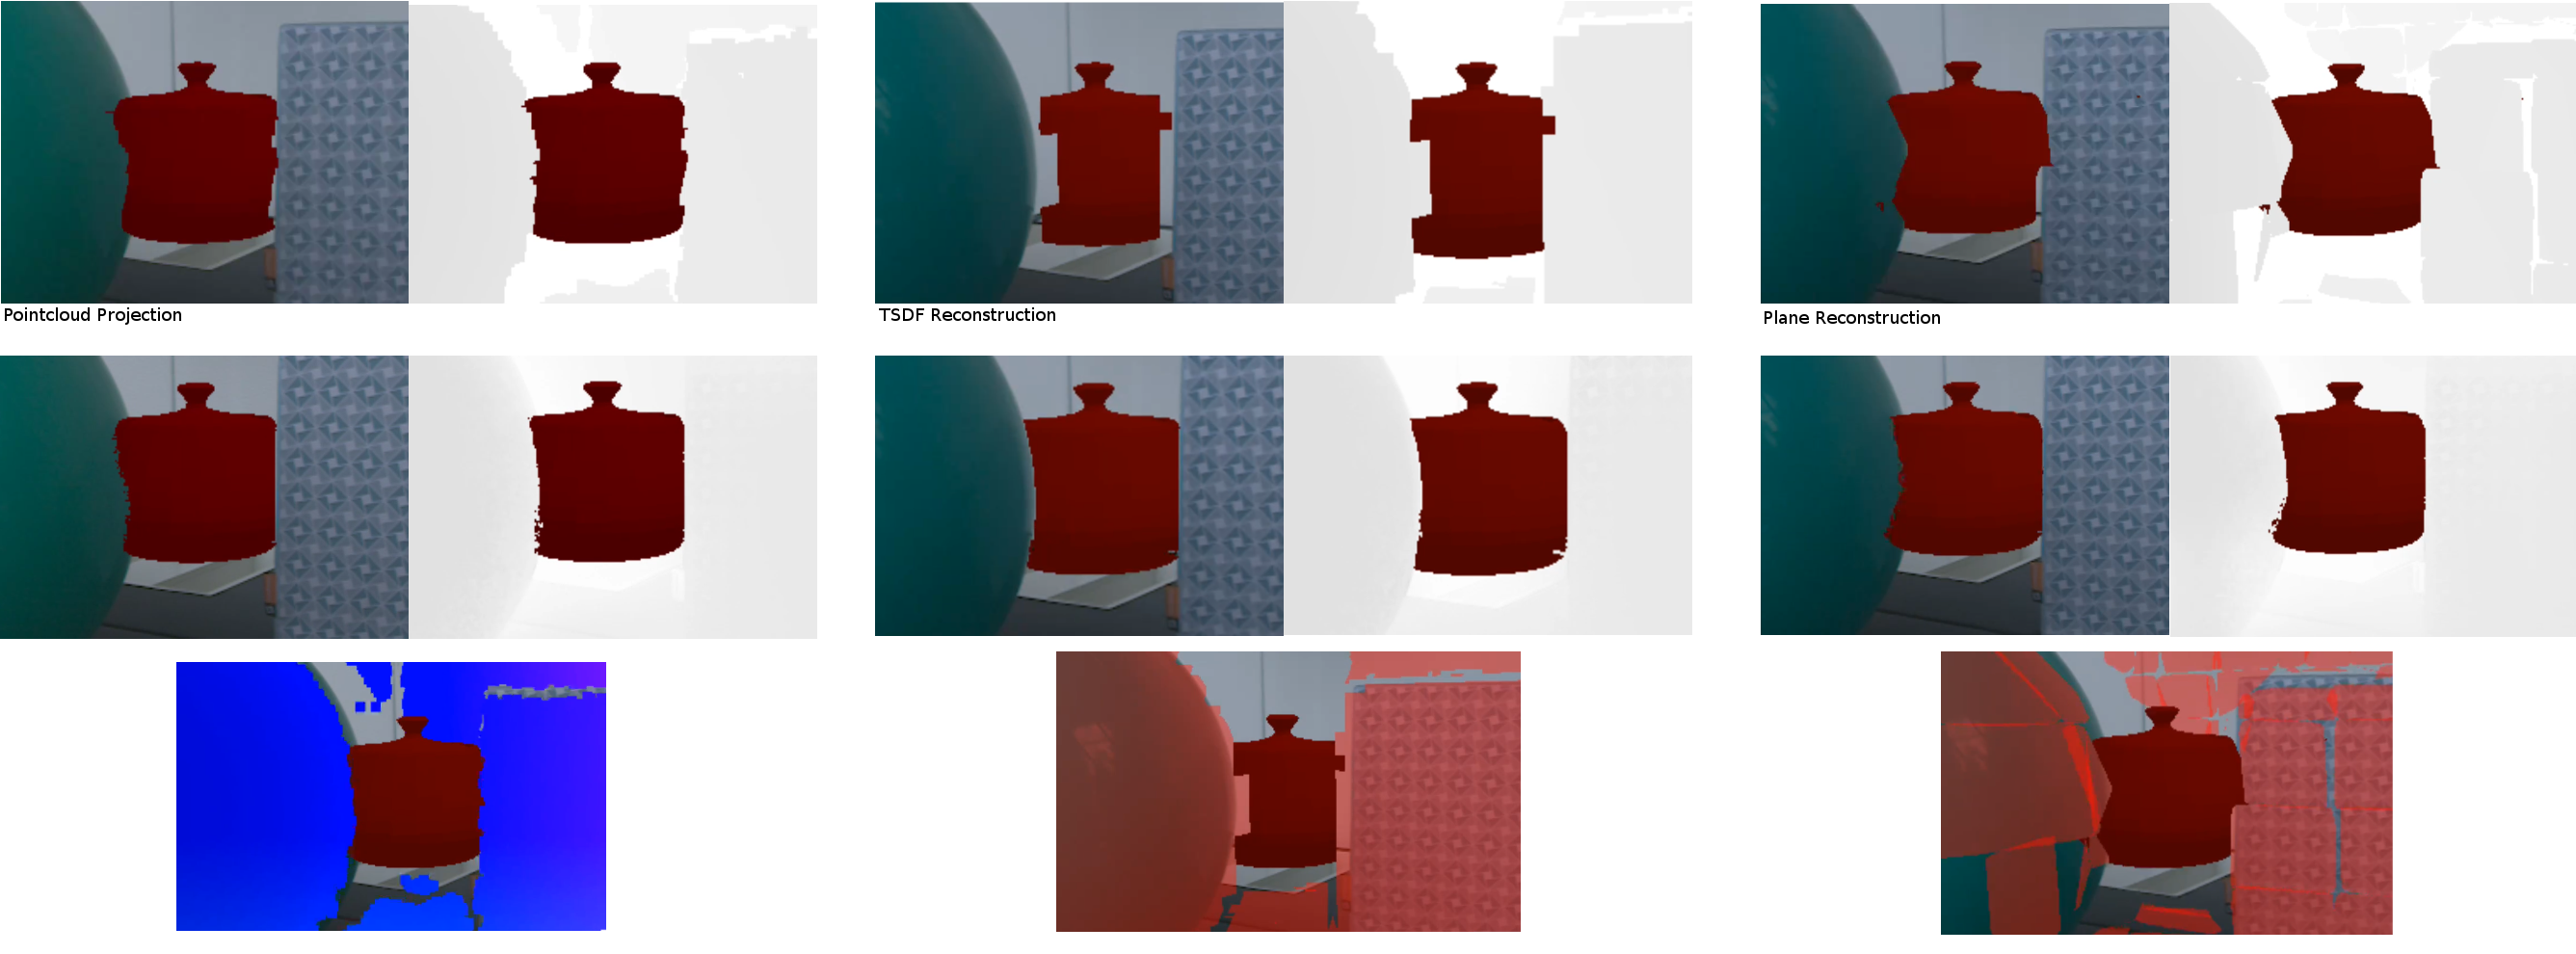
\includegraphics[width=1.0\textwidth]{content/images/evaluation/static_occlusion.png} 
  \caption{Ergebnisaufnahmen aus der ersten statischen Szene}
  \label{fig:static_occlusion}
\end{sidewaysfigure}

\begin{sidewaysfigure}[h]
  \centering
	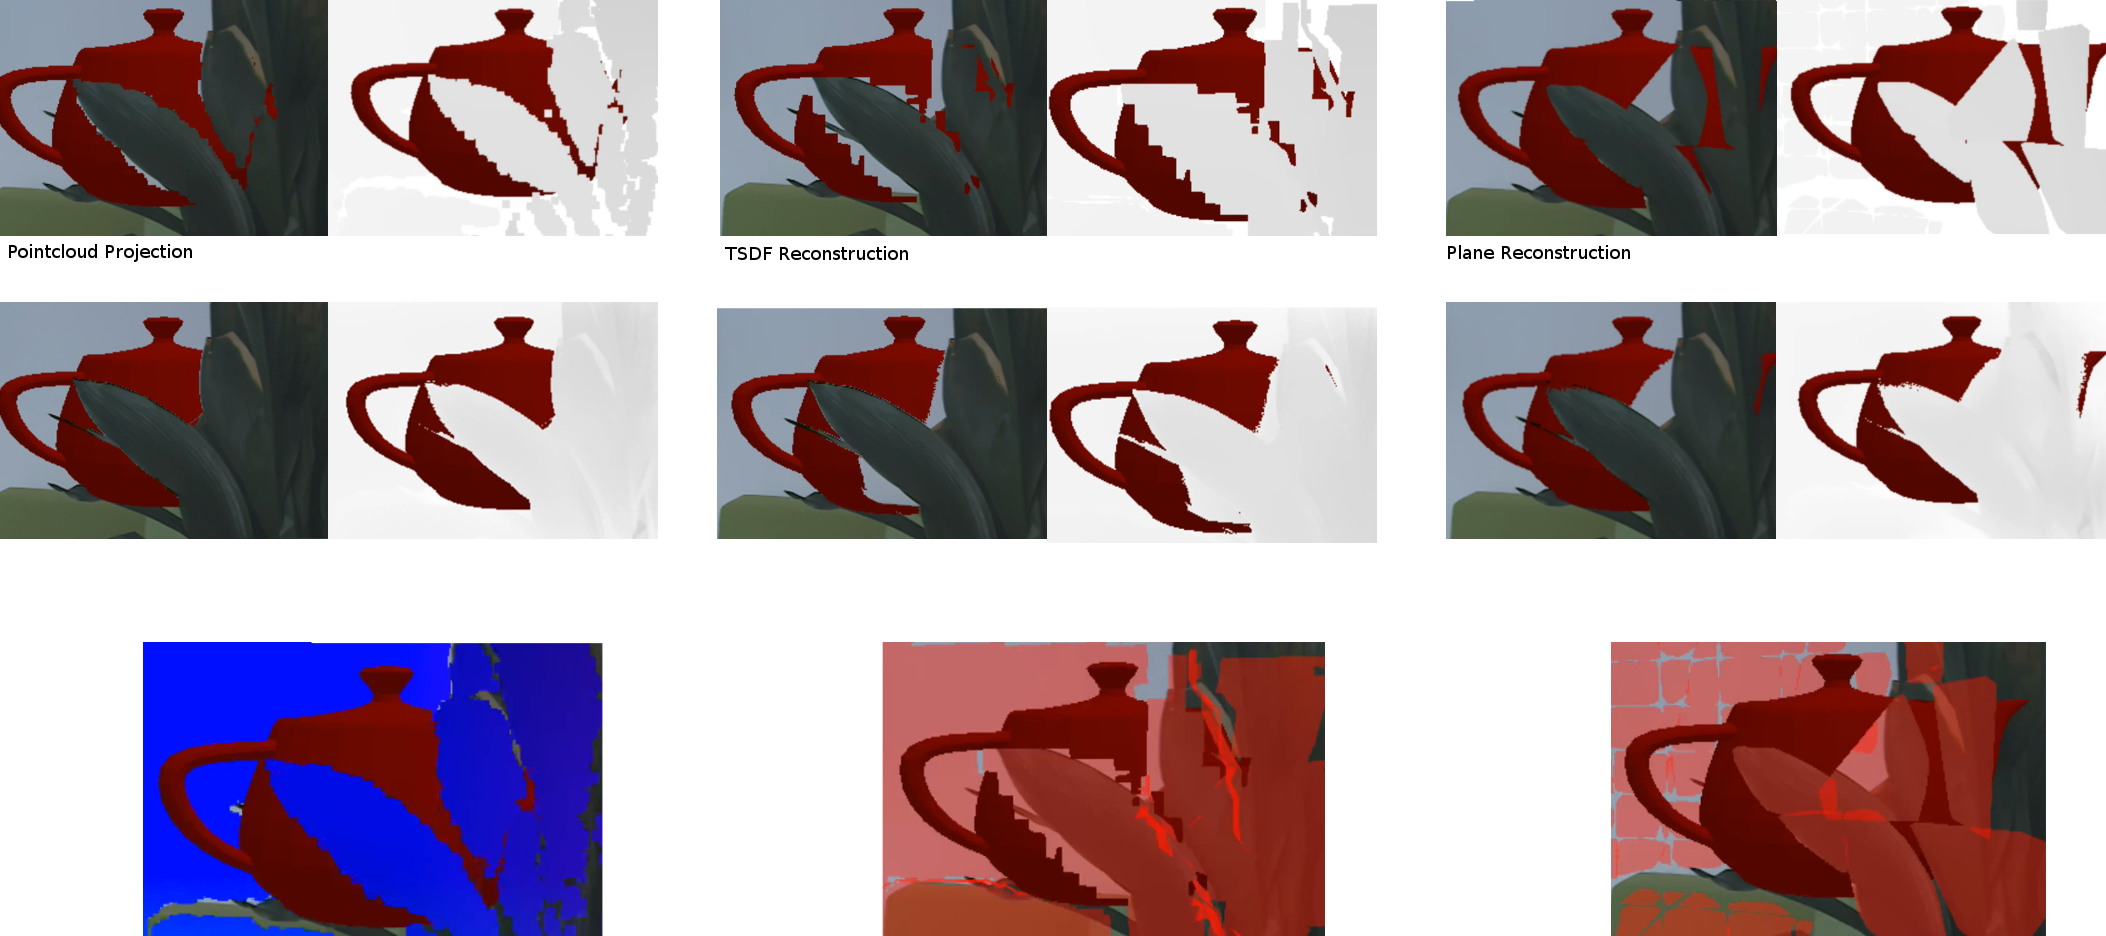
\includegraphics[width=1.0\textwidth]{content/images/evaluation/plant_occlusion.png} 
  \caption{Ergebnisaufnahmen aus der zweiten statischen Szene}
  \label{fig:plant_occlusion}
\end{sidewaysfigure}

\begin{sidewaysfigure}[h]
  \centering
	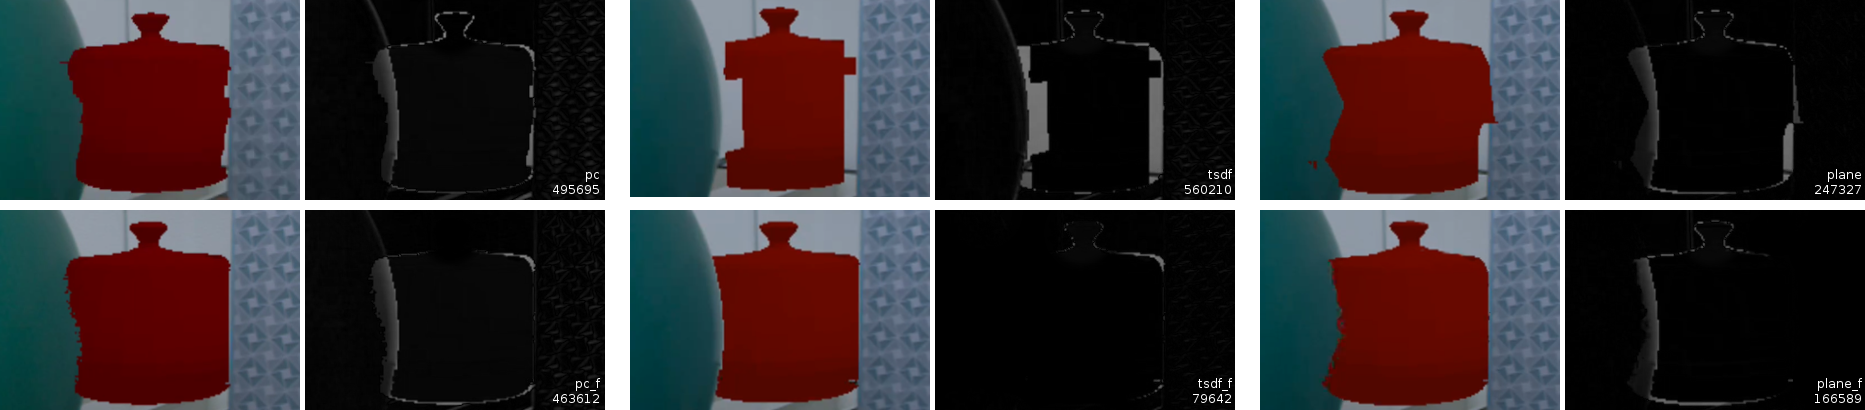
\includegraphics[width=1.0\textwidth]{content/images/evaluation/static_occlusion_results.png} 
	
\includegraphics[width=1.0\textwidth]{content/images/evaluation/spacer.png} 
	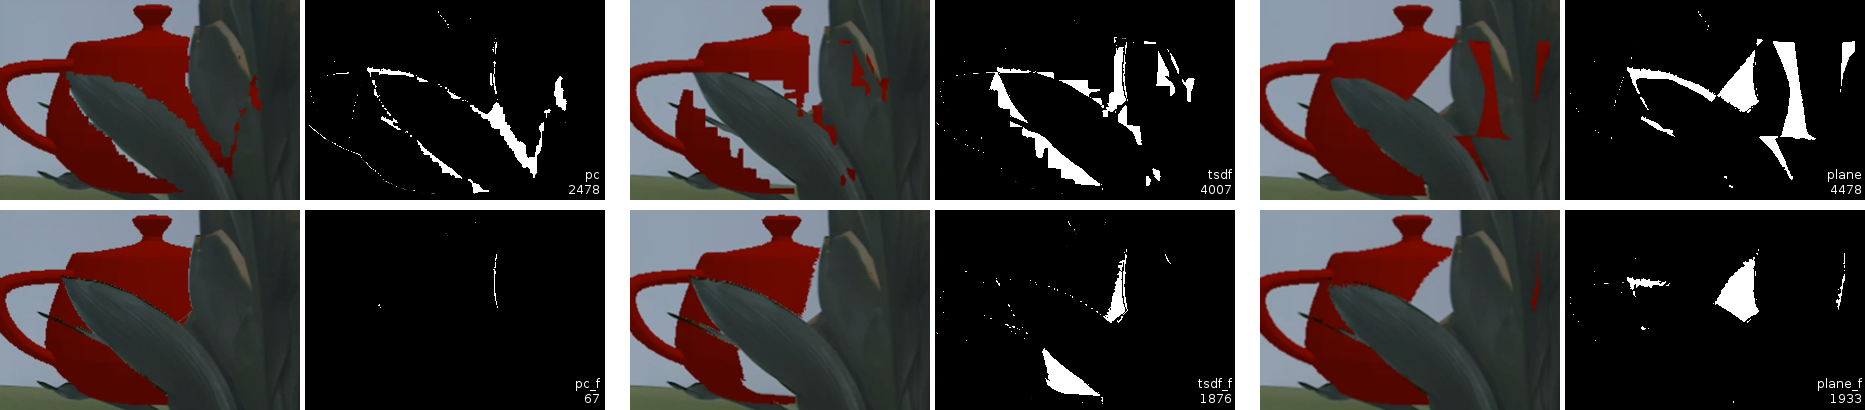
\includegraphics[width=1.0\textwidth]{content/images/evaluation/plant_occlusion_results.png} 
  \caption{Differenzbilder der Verfahren in ersten (oben) und zweiten Szene (unten)}
  \label{fig:static_occlusion_results}
\end{sidewaysfigure}

\chapter{Differenz OpenCV Python Skript}

\begin{lstlisting}[mathescape,caption=Python Implementierung der Bilddifferenz, label=lst:compare, language=Python]
from cv2 import *
from os import listdir
from os.path import isfile, join

reference_path = "reference.png"
reference = imread(reference_path)
reference = cvtColor(reference, COLOR_BGR2GRAY)
all_images = [f for f in listdir("./") 
    if isfile(join("./", f)) and f.endswith(".png")]
    
for img_path in all_images:
    img = imread(img_path)
    img = cvtColor(img, COLOR_BGR2GRAY)
    result = absdiff(reference, img)
    imwrite("result_" + img_path, result)
    difference = sumElems(result)
    print str(int(result[2])) + "\t" + result[0] + "\t" + result[1]
\end{lstlisting}